\section{Results}

In this section, we present the numerical results obtained from the
implementation, including total cross sections and differential
distributions.

\subsection{Total cross sections}

The NLO cross section for $pp \to t\bar{t}$ was computed at two
center-of-mass energies, using the NNPDF3.1 NLO PDF set with
$\alpha_s = 0.118$ and renormalization and factorization scales
set to $\mu_R = \mu_F = m_t = 173~\text{GeV}$.

At $\sqrt{s} = 8~\text{TeV}$, we obtain:
\begin{align}
\sigma_{\text{NLO}} = 220.666 \pm 0.552~\text{pb},
\end{align}
to be compared with the Top++ prediction:
\begin{align}
\sigma_{\text{Top++}} = 220.689~\text{pb}.
\end{align}

At $\sqrt{s} = 13~\text{TeV}$, we obtain:
\begin{align}
\sigma_{\text{NLO}} = 731.972 \pm 0.6211~\text{pb},
\end{align}
to be compared with:
\begin{align}
\sigma_{\text{Top++}} = 732.912~\text{pb}.
\end{align}

The agreement at the level of $\mathcal{O}(10^{-2})$ pb demonstrates
the correctness of the implementation and the normalization.

\subsection{Differential distributions}

We also computed several differential distributions at LO and NLO
and compared them with reference results.

\subsubsection{Invariant mass distribution}

The invariant mass distribution of the top-quark pair is shown in
Fig.~\ref{fig:mtt_lo} and Fig.~\ref{fig:mtt_nlo}.

\begin{figure}[h!]
\centering
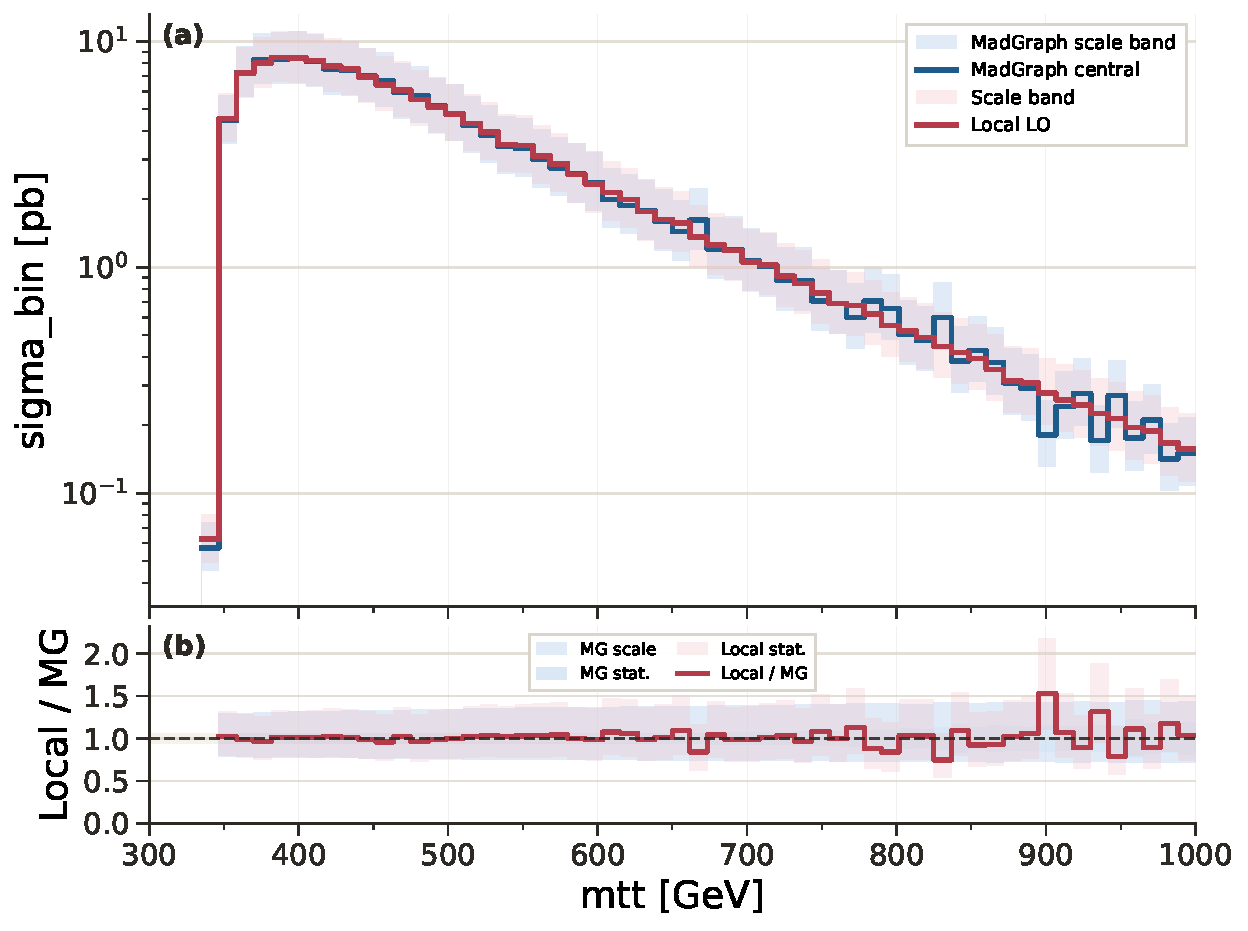
\includegraphics[width=0.4\textwidth]{figures/mtt_lo_vs_madgraph.pdf}
\caption{Invariant mass distribution at LO compared to MadGraph.}
\label{fig:mtt_lo}
\end{figure}

\begin{figure}[h!]
\centering
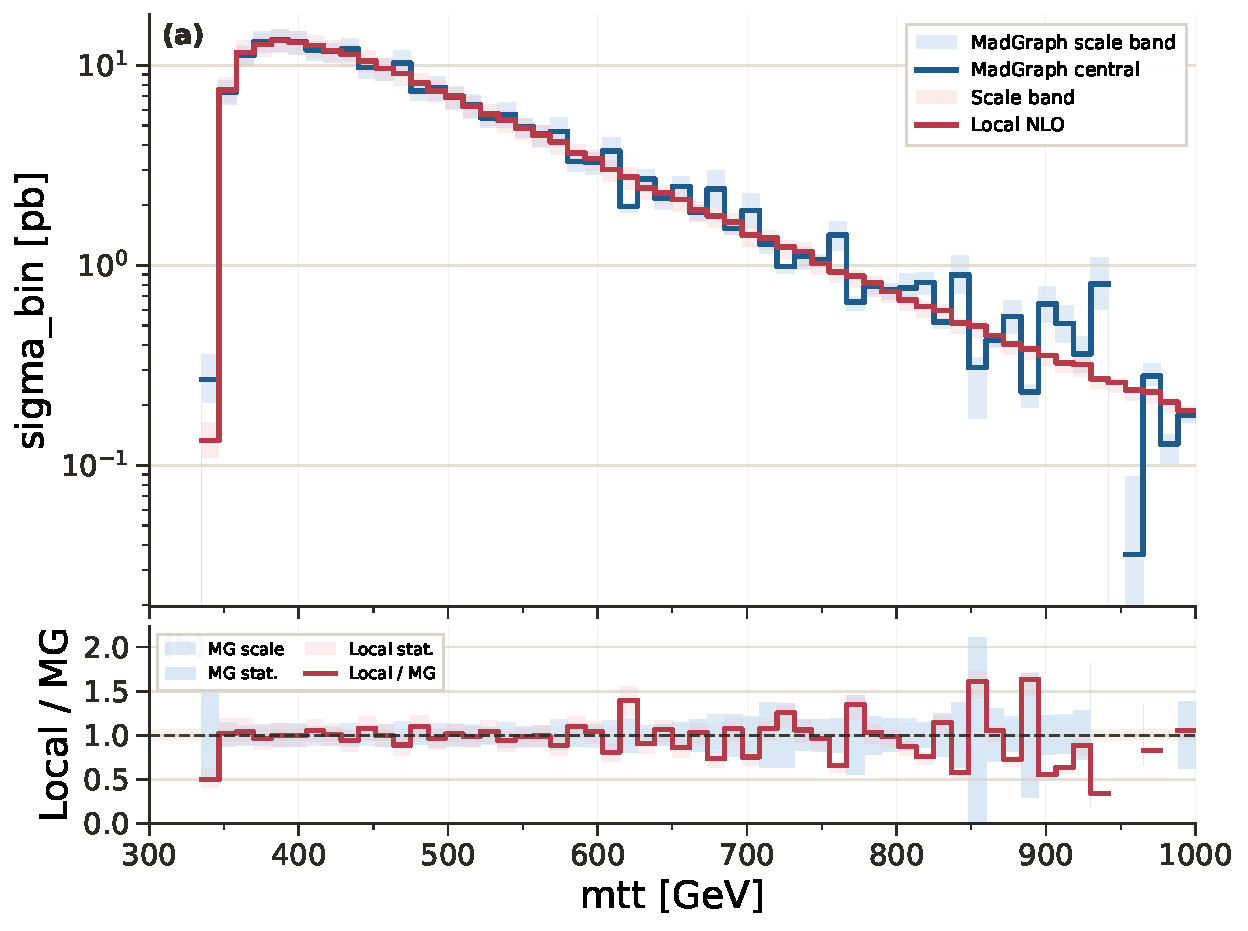
\includegraphics[width=0.4\textwidth]{figures/mtt_nlo_vs_madgraph.pdf}
\caption{Invariant mass distribution at NLO compared to reference results.}
\label{fig:mtt_nlo}
\end{figure}

\subsubsection{Top transverse momentum}

The transverse momentum distribution of the top quark is shown in
Fig.~\ref{fig:pt_lo} and Fig.~\ref{fig:pt_nlo}.

\begin{figure}[h!]
\centering
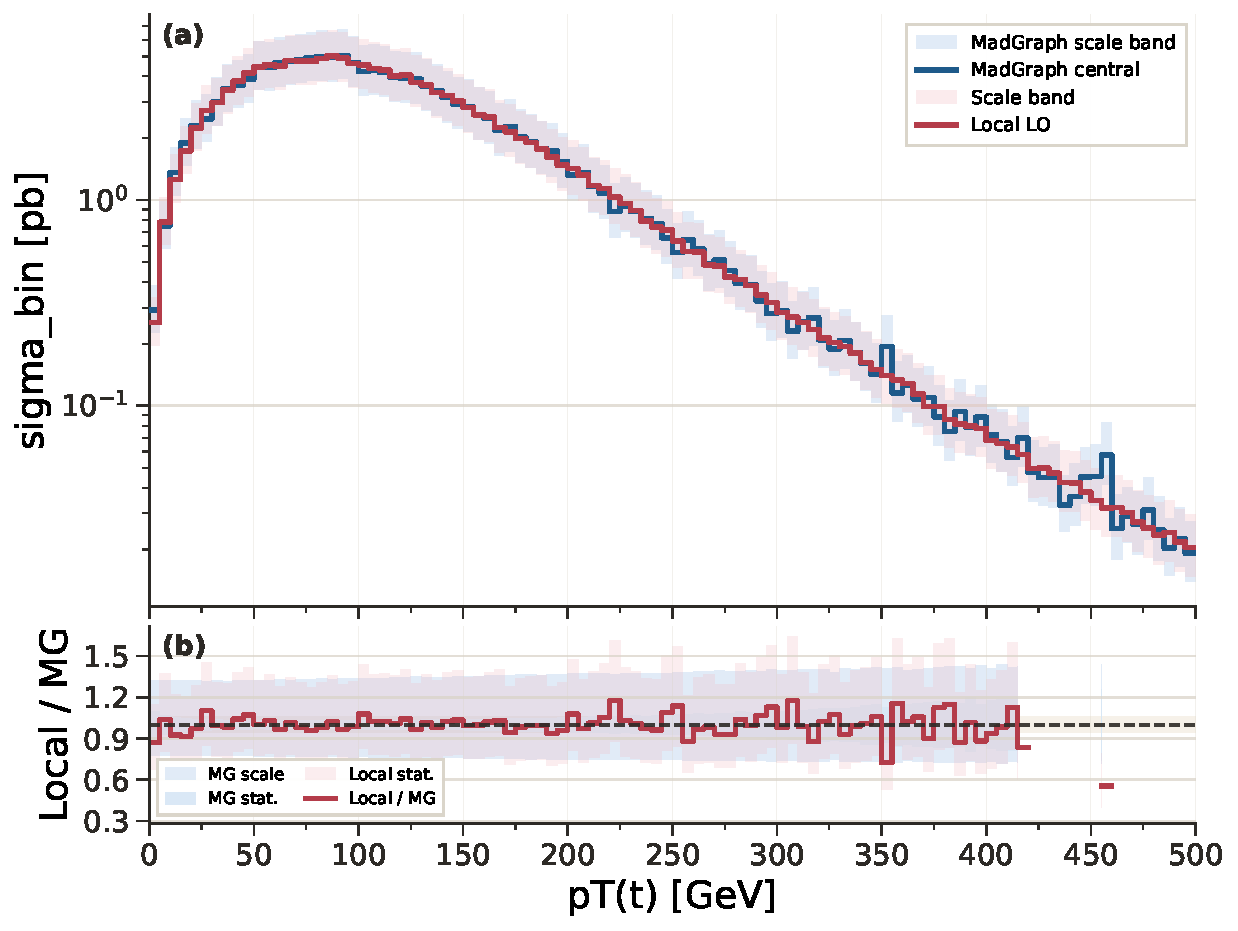
\includegraphics[width=0.4\textwidth]{figures/top_pt_lo_vs_madgraph.pdf}
\caption{Top $p_T$ distribution at LO compared to MadGraph.}
\label{fig:pt_lo}
\end{figure}

\begin{figure}[h!]
\centering
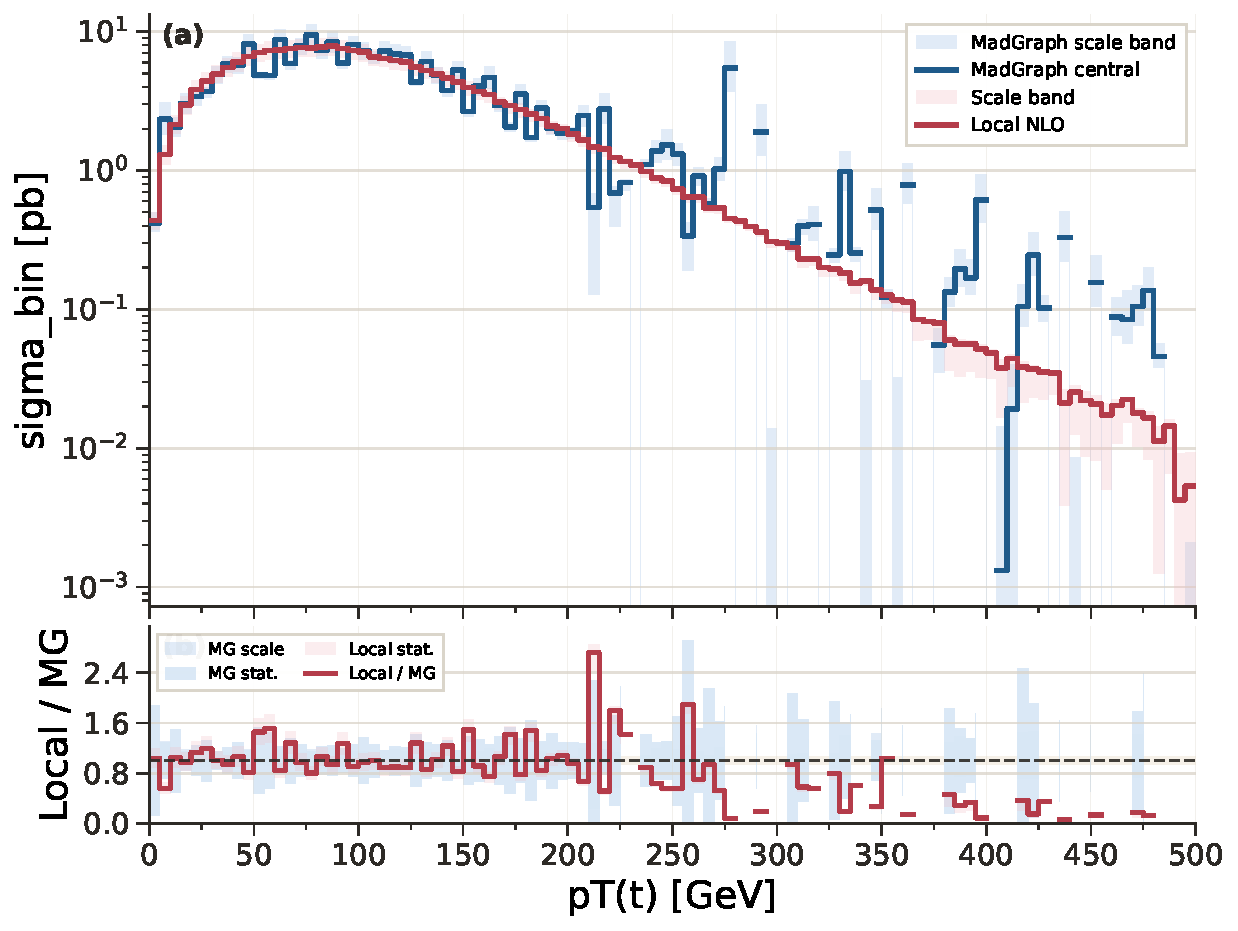
\includegraphics[width=0.4\textwidth]{figures/top_pt_nlo_vs_madgraph.pdf}
\caption{Top $p_T$ distribution at NLO.}
\label{fig:pt_nlo}
\end{figure}

\subsubsection{Rapidity distribution}

The rapidity distribution of the $t\bar{t}$ system is shown in
Fig.~\ref{fig:ytt_lo} and Fig.~\ref{fig:ytt_nlo}.

\begin{figure}[h!]
\centering
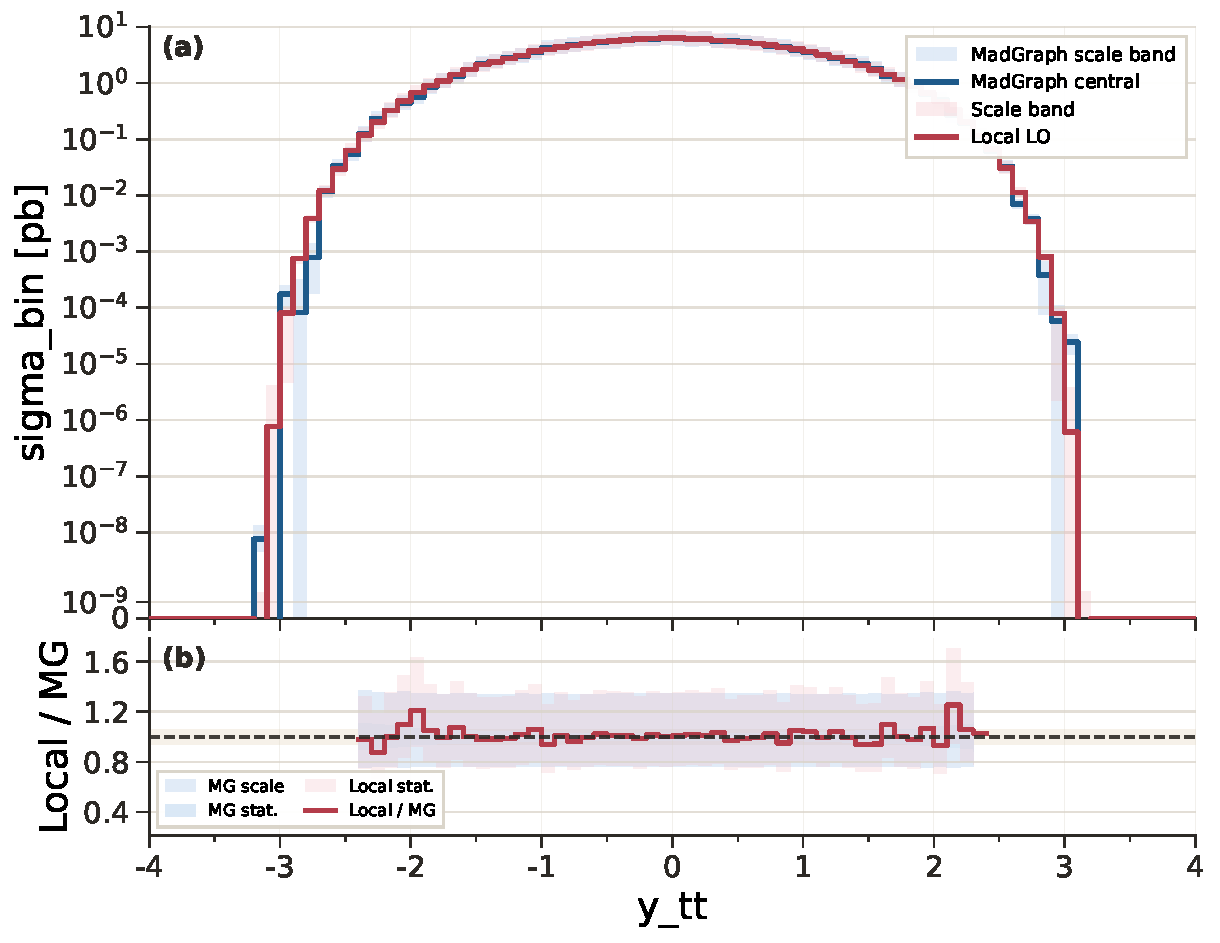
\includegraphics[width=0.4\textwidth]{figures/ytt_lo_vs_madgraph.pdf}
\caption{Rapidity distribution at LO.}
\label{fig:ytt_lo}
\end{figure}

\begin{figure}[h!]
\centering
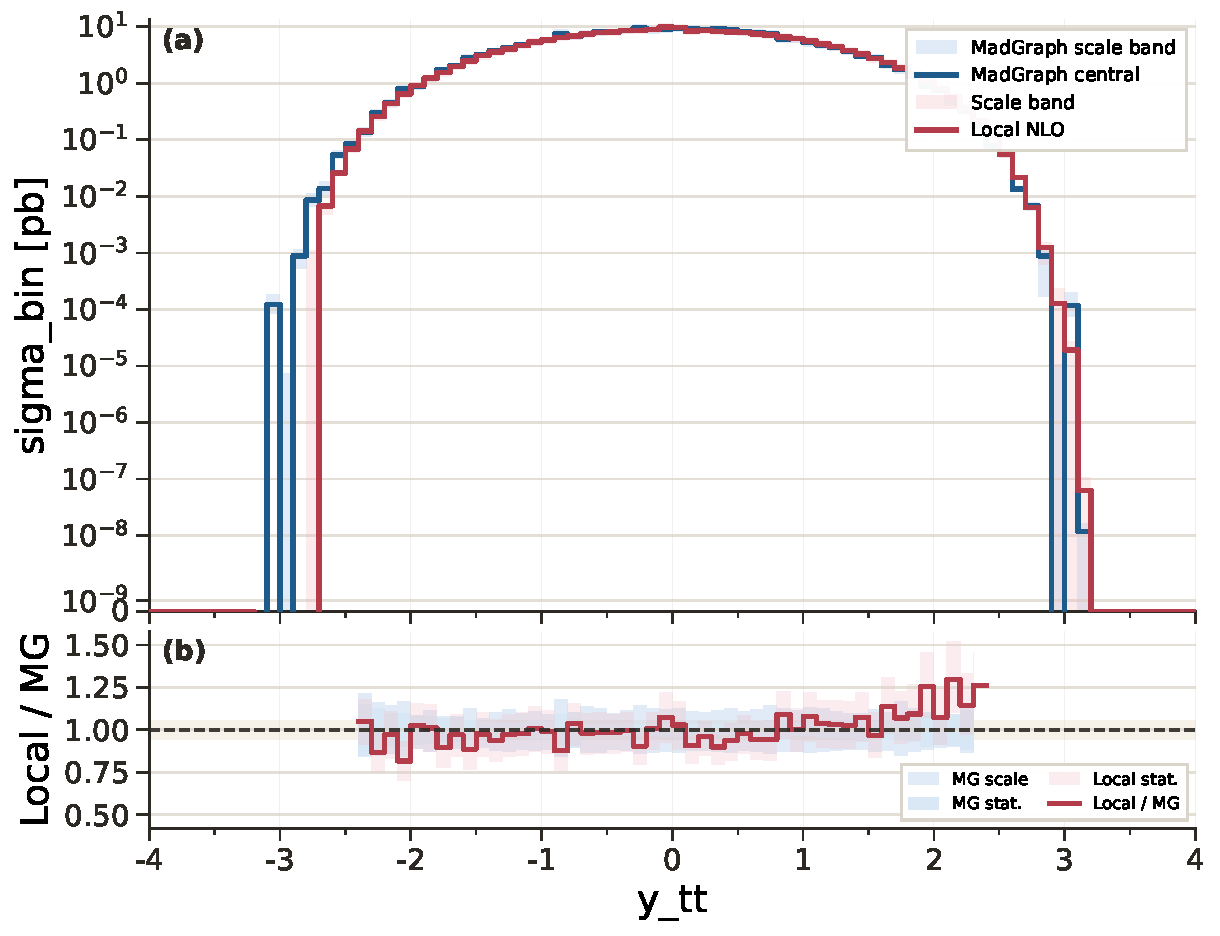
\includegraphics[width=0.4\textwidth]{figures/ytt_nlo_vs_madgraph.pdf}
\caption{Rapidity distribution at NLO.}
\label{fig:ytt_nlo}
\end{figure}

\subsection{Discussion}

The total cross sections show excellent agreement with Top++,
indicating that both the normalization and the subtraction procedure
are correctly implemented.

At the differential level:
\begin{itemize}
    \item LO distributions agree with MadGraph, validating the phase-space
    generation and matrix elements,
    \item NLO corrections modify both normalization and shape,
    \item the distributions remain smooth, confirming numerical stability.
\end{itemize}

Overall, these results demonstrate that the implementation correctly
reproduces both inclusive and differential observables at NLO.